\subsection{Implementationsarkitektur}
Implementationsarkitekturen ger en mer detaljerad beskrivning över systemet som ligger till grund för den konkreta implementationen. Arkitekturen är här uppdelad i UI-applikation och kontroll-applikation för tydlighet. Komponenten IoT-Backend har utelämnats ur modellerna då den inte innehåller några relevanta arkitekturbeslut. Use case maps och impact maps över implementationsarkitekturen kan hittas i appendix \ref{sec:use_case_implementation} respektive \ref{sec:impact_implementation}.

\subsubsection{Modell UI-Applikation}
Figur \ref{fig:implementationsarkitektur-UI} visar en modell över implementationsarkitekturen för UI-Applikationen. Kommunikationen från komponenten benämnd UI-kommunikation går till den IoT-Backend som presenteras i konceptarkitekturen. Denna är här utelämnad för tydlighet. Streckade rutor är grupperingar av komponenter som utgör stora delar i systemet. Gränssnittet mellan spel och spelläge ska betraktas som en viktig informationsväg och inte en självstående komponent.

\begin{figure}[h]
    \centering
    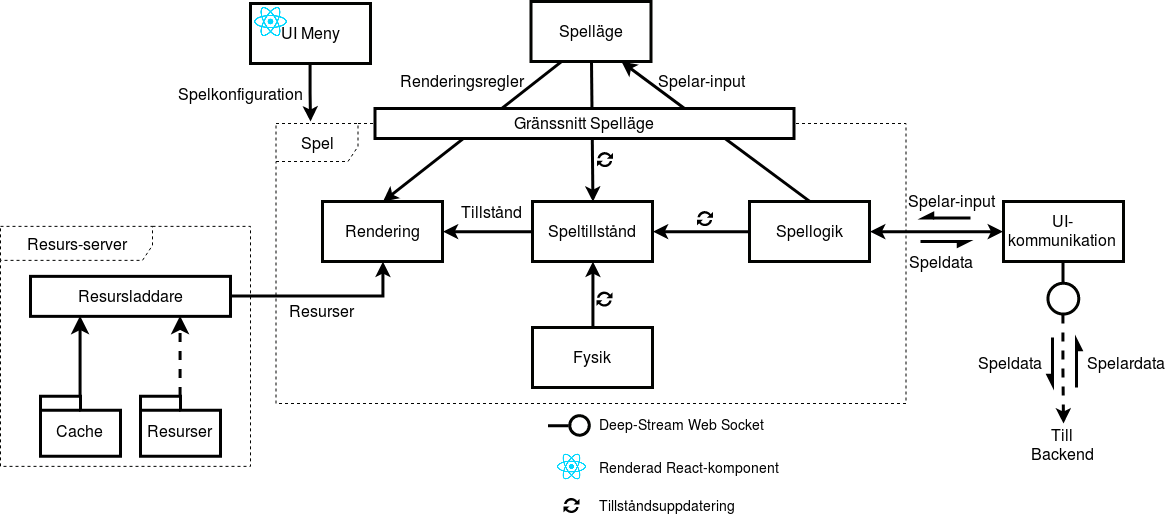
\includegraphics[scale=0.4]{implementationsarkitektur_UI}
    \caption{Modell över implementationsarkitektur för UI-Applikationen}
    \label{fig:implementationsarkitektur-UI}
\end{figure}

\subsubsection{Implementationsbeskrivning}
\label{subsubsec:implementation-desc-UI}
UI-Applikationen har till stor del förfinats från den mer övergripande modellen i konceptarkitekturen. Främst är det spelkomponenten som har delats upp i sina beståndsdelar. Även resurs-servern har förtydligats och ett specifikt gränssnitt mellan spel och spelläge införts.\\

Implementationsarkitekturen innehåller några tekniska detaljer som är viktiga för arkitekturens uppbyggnad. Använding av React för rendering av vissa komponenter är förtydligat i modellen. Detta tillåter välstrukturerade menyer och hårt definierade gränser mellan komponenter. Även kommunikationssystemet Deep Stream är utmarkerat i modellen. Deep Stream är robust nog för de kommunikationskrav som är centrala för arkitekturen. Det innehåller också funktionalitet som gör att utvecklingen av nätverksdelarna inte behöver fokuseras alltför mycket på detaljerad optimering.\\

\subsubsection{Spelet}
Spelet, som är den centrala delen i UI-applikationen, är i denna modell uppdelad i flera mindre komponenter. Detta möjliggör en mer strukturerad syn på systemet och bättre möjligheter att definiera gränssnittet mellan spellägen och grundspelet. Centralt i spelet är tillståndet, som kan läsas av och muteras från flera av de andra komponenterna. Fysikkomponenten ändrar speltillståndet baserat på de implementerade fysikreglerna. Spellogiken tar spelarnas handlingar och för spelet framåt baserat på den mest grundläggande spelmekaniken. För att presentera spelet för användare sker rendering baserat på spelets nuvarande tillstånd. I denna rendering används också de resurser som laddas genom resurs-servern. Modellen visar hur data flödar mellan spelets interna komponenter i ordning. Ur ett exekveringsperspektiv skulle varje komponent vara en mindre del i en stor spelloop. Denna spelloop är det som driver data från spelar-input, genom systemet, till rendering.\\

Med denna mer detaljerade design är det möjligt att tydligare definiera gränssnittet mellan grundspelet och spelläget. Detta är centralt för att göra det möjligt att utveckla många olika intressanta spellägen samtidigt som en effektiv, modulär arkitektur bibehålls. Spelläget kan genom detta gränssnitt direkt påverka spelets tillstånd, men även sätta regler för renderingen. Genom att spellogiken skickar nya händelser ut till spelläget kan förändringar baserade på spelares handlingar utföras specifikt för det valda spelläget. Konkret i implementationen kan detta ske genom funktioner i spelläget som injiceras i spellogiken. Spellägets påverkan på renderingen är nödvändig för att ge spellägen större kontroll över spelets grafiska utseende. Exempel på sådan påverkan kan vara renderingseffekter eller utritning av spelinformation specifik för det valda spelläget. Med detta gränssnitt blir det tydligt att det finns goda möjligheter att utveckla många olika spellägen.\\

\subsubsection{Hjälpkomponenter}
Resurs-servern består i denna modell av flera interagerande komponenter. Detta ska illustrera dess viktiga roll i att se till att endast nödvändiga resurser behöver laddas. Resursladdaren ska ses som logik för detta. Cache och Resurser representerar lagringen av resurser lokalt och på server. Förhoppningen är att denna komponent ska effektivisera systemet genom att undvika onödig inladdning av resurser.\\

Menyn i UI-Applikationen, som är en renderad React-komponent, har i denna modell som främsta uppgift att ta fram den konfiguration som spelsessionen ska använda sig av. Den erbjuder användaren menyalternativ för att välja detta och skapar sedan spelet utifrån denna konfiguration. Spelet ansvarar sedan för att sätta upp kommunikationen och starta spelsessionen. Med denna struktur begränsas antalet anslutningar mellan olika komponenter i UI-applikationen, vilket leder till en mer modulär och utökningsbar arkitektur.\\

\subsubsection{Modell Kontroll-Applikation}
Implementationsarkitekturen för kontroll-applikationen presenteras i figur \ref{fig:implementationsarkitektur-kontroll}. Även denna följer samma notation som för UI-applikationen. Resurs-servern är identisk med samma komponent i UI-delen.

\begin{figure}[h]
    \centering
    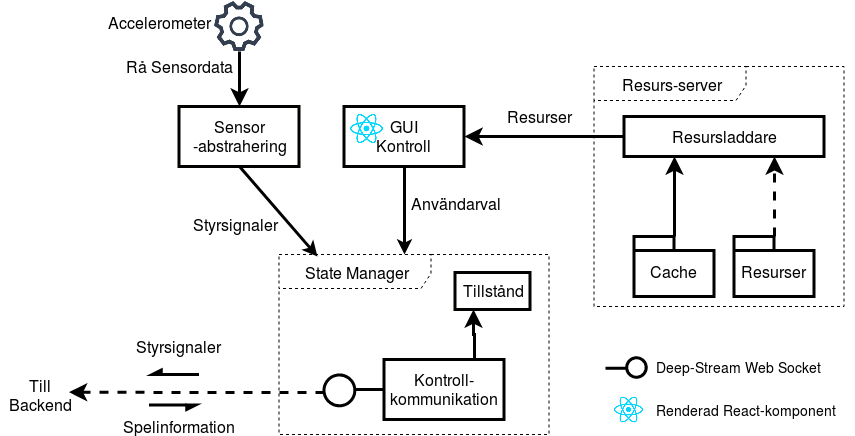
\includegraphics[scale=0.4]{implementationsarkitektur_kontroll}
    \caption{Modell över implementationsarkitektur för kontroll-applikationen}
    \label{fig:implementationsarkitektur-kontroll}
\end{figure}

\subsubsection{Beskrivning Kontroll-Applikation}
Implementationsarkitekturen för kontroll-applikationen innehåller liknande idéer och uppdelningar som UI-applikationen. Även här finns förtydliganden av tekniska detaljer. För ytterligare information och motivationer för dessa se \ref{subsubsec:implementation-desc-UI}.\\

Sensoravläsningen är i denna modell uppdelad i accelerometer och dataabstrahering. Accelerometerdelen består av den färdiga hårdvara och mjukvara som tillåter åtkomst till rå data från sensorn. Abstraheringen standardiserar denna data och skickar den vidare mot kommunikationsdelen.\\

Den stora del som benämns State Manager är en utveckling av kommunikationsdelen på kontroll-applikationen för att styra mer av programmets tillstånd. Tillståndet i denna komponent representerar saker som huruvida uppkopplingen är aktiv och vilket spelläge som körs. Detta styr sedan operationen hos andra komponenter. Genom att lägga detta tillstånd nära kommunikationsdelen, som kan ses som den tyngsta komponenten i kontrollen, är idén att bibehålla lätta, korta informationsvägar. Detta introducerar inte heller fler, onödiga komponenter som motverkar målet att hålla kontroll-applikationen tunn.\\
